\iffalse
\documentclass[journal,10pt,twocolumn]{article}
\usepackage{graphicx, float}
\usepackage[margin=0.5in]{geometry}
\usepackage{amsmath, bm}
\usepackage{array}
\usepackage{booktabs}

\providecommand{\norm}[1]{\left\lVert#1\right\rVert}
\let\vec\mathbf
\newcommand{\myvec}[1]{\ensuremath{\begin{pmatrix}#1\end{pmatrix}}}
\newcommand{\mydet}[1]{\ensuremath{\begin{vmatrix}#1\end{vmatrix}}}

\title{\textbf{Line Assignment}}
\author{YOGEESH REDDY}
\date{September 2022}

\begin{document}

\maketitle
\paragraph{\textit{\large Problem Statement} -
\fi
The perpendicular from the origin to a line meets it at the point (-2,9). Find the equation of the line.
	\begin{figure}[!ht]
		\centering
 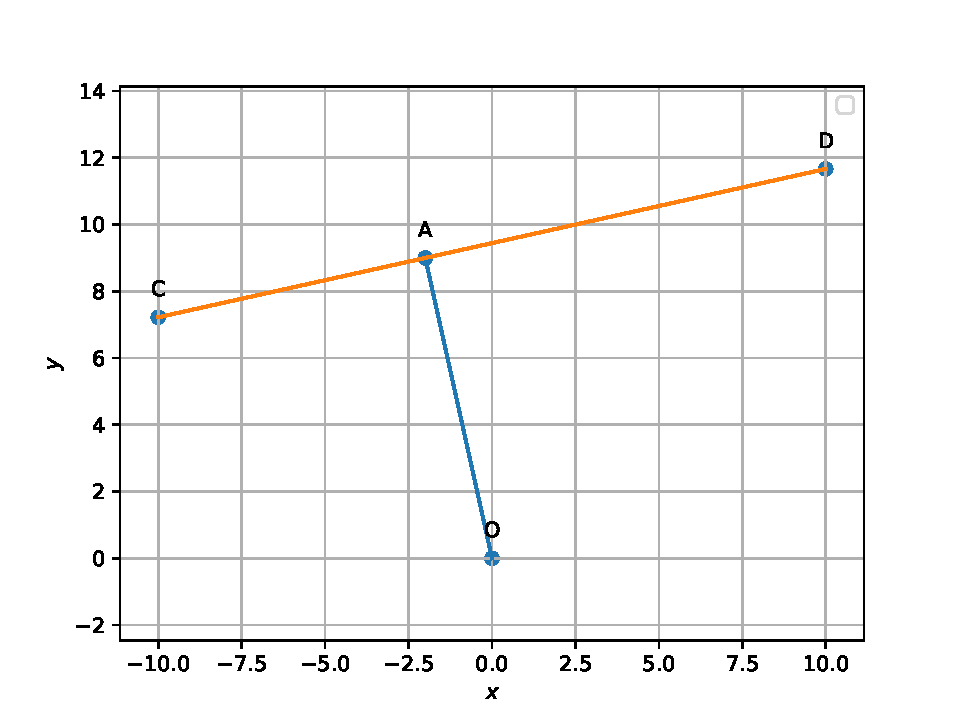
\includegraphics[width=\columnwidth]{chapters/11/10/2/15/figs/line.pdf}
		\caption{}
		\label{fig:11/10/2/15}
  	\end{figure}
	\\
	\solution
	\iffalse
\section*{\large Solution}
\begin{figure}[H]
\centering
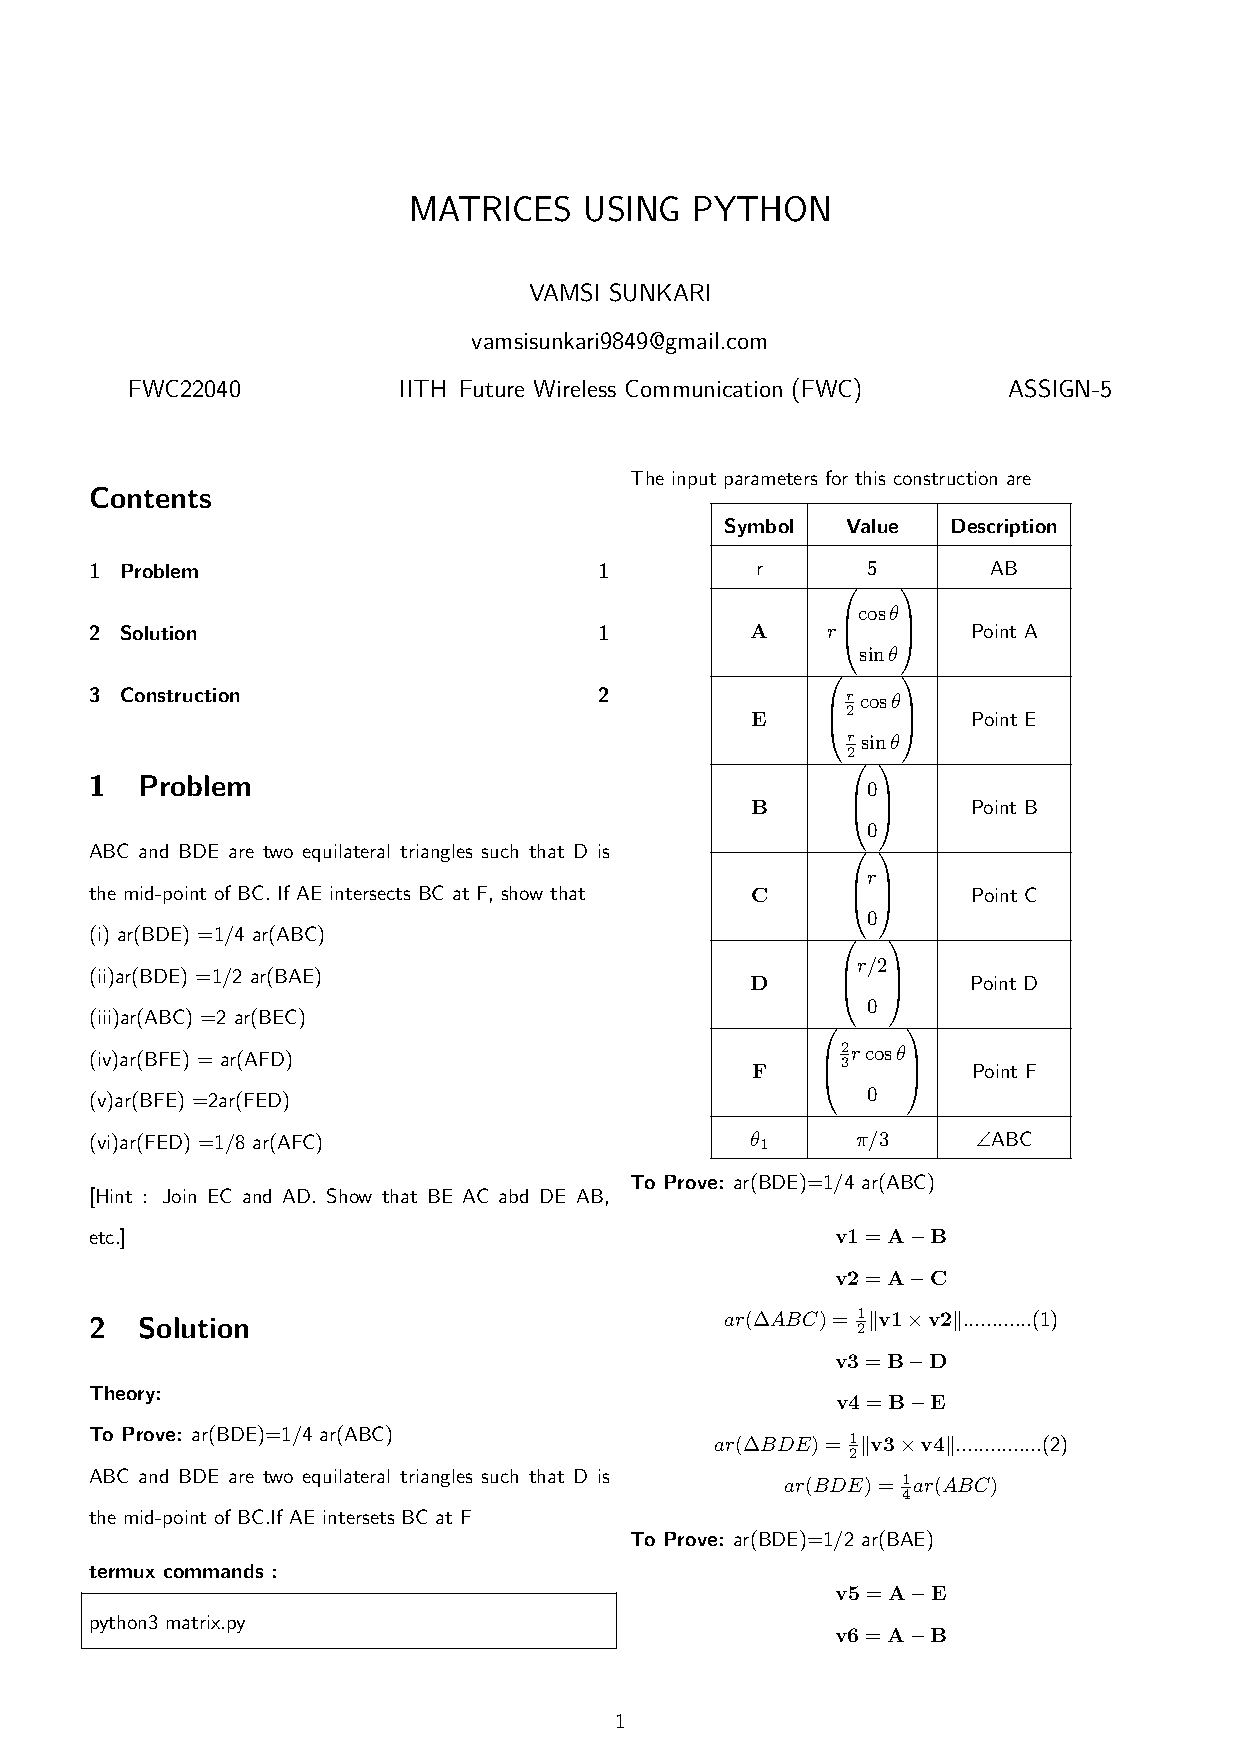
\includegraphics[width=1\columnwidth]{matrix.pdf}
\caption{}
\end{figure}

\section*{\large Construction}



The input parameters of figure 



\begin{table}[htbp]
 \begin{center}
    \begin{tabular}{|l|c|c|c|c|c|c} \hline \textbf{Symbol}
  & \textbf{value} \\
 \hline
O & $\myvec{0\\0}$ \\ \hline
A & $\myvec{-2\\9}$  \\ \hline
D &  $\myvec{x\\y}$  \\ \hline

 
\end{tabular}   
\end{center}
\caption{\label{table:dummytable} }
\end{table}

\vspace*{10mm}


\section*{Solution:}
\fi

Given 
\begin{align}
 \vec{0} = \myvec{0\\0},
 \vec{A} = \myvec{-2\\9}
\end{align}
\iffalse
Let D be a point on the required line :
\begin{align}
 \vec{D} = \myvec{x\\y}
\end{align} 
 \begin{align}
 \vec{D-A}=\myvec{x+2\\y-9}
   \end{align}
   \fi
   The 
normal vector is
\begin{align}
	\vec{n}&=\vec{O}- \vec{A}
	\\
	&=\myvec{2\\-9}
\end{align}
yielding the equation of the line as

\begin{align}
	\myvec{2 & -9}\brak{\vec{x} - \myvec{2 \\ -9}}&= 0
	\\
	\implies 
	\myvec{2 & -9}\vec{x} &= 85
\end{align}
\iffalse

\begin{align}
 2\vec{x}-9\vec{y}+85=0
\end{align}


\end{document}
\fi
